% Suggested filename: bananas.tex
\documentclass[12pt]{article}

%========== (1) Math Packages ==========
\usepackage{amsmath,amssymb,amsthm}

%========== (2) General Packages: Hebrew support, fonts, etc ==========
\usepackage{xcolor}
\usepackage{float}
\usepackage{graphicx}
\usepackage{hyperref}
\usepackage{booktabs}
\usepackage{enumerate}
\usepackage{fancyvrb}
\usepackage{fancyhdr}
\usepackage{setspace}
\usepackage[most]{tcolorbox}

\usepackage{fontspec}
\usepackage{polyglossia}

\newcommand{\enquote}[1]{\textquotedblleft #1\textquotedblright}

% Language settings
\setdefaultlanguage{hebrew}
\setotherlanguage{english}

% Fonts
% Using Narkisim as an alternative Hebrew font for body text for variety, David CLM for TT
\newfontfamily\hebrewfont[Script=Hebrew]{Narkisim}
\newfontfamily\englishfont{Times New Roman}
\newfontfamily\hebrewfonttt[Script=Hebrew]{David CLM} % Keeping David CLM for monospace if needed

% Hyperref link color settings (changed to black as requested by implied constraint)
\hypersetup{
  colorlinks=true,
  linkcolor=black,
  urlcolor=black,
  citecolor=black
}

% Table of Contents setup
\usepackage{tocloft}
\usepackage{etoolbox}

\makeatletter
\renewcommand\tableofcontents{\section*{\contentsname}
    @starttoc{toc}}
\makeatother

%========== Spacing and Paragraphs ==========
\onehalfspacing
\setlength{\parskip}{6pt}
\setlength{\parindent}{0pt}

%========== Header/Footer Settings ==========
\pagestyle{fancy}
\setlength{\headheight}{14.5pt}
\addtolength{\topmargin}{-2.5pt}
\fancyhf{}
\lhead{מידע על בננות} % Changed from placeholder
\rhead{\today} % Keep date on the right
\cfoot{\thepage} % Page number in the center

%========== tcolorbox Setup ==========
% Adjusted colors slightly to be less pale as requested
\tcbset{
  boxsep=5pt,
  top=5pt, bottom=5pt, left=5pt, right=5pt,
  middle=5pt,
  sharp corners % Keeping sharp corners for a clean look as per example
}

%========== Special Boxes: Definition, Remark, Example ==========
\newtcolorbox{definitionBox}[1]{
  title=\textbf{#1}, % Make title bold
  colback=green!8!white, % Slightly more saturated green
  colframe=green!50!black,
  enhanced % For rounded corners if needed later, but keeping sharp corners per tcbset
}

\newtcolorbox{remarkBox}[1]{
  title=\textbf{#1}, % Make title bold
  colback=yellow!8!white, % Slightly more saturated yellow
  colframe=yellow!50!black,
  enhanced
}

\newtcolorbox{exampleBox}[1]{
  title=\textbf{#1}, % Make title bold
  colback=red!8!white, % Slightly more saturated red
  colframe=red!50!black,
  enhanced
}

% Define other potential boxes mentioned
\newtcolorbox{lawBox}[1]{
  title=\textbf{#1}, % Make title bold
  colback=blue!8!white, % Slightly more saturated blue
  colframe=blue!50!black,
  enhanced
}

\newtcolorbox{resultBox}[1]{
  title=\textbf{#1}, % Make title bold
  colback=orange!8!white, % Slightly more saturated orange
  colframe=orange!50!black,
  enhanced
}


% Bullet fix for Hebrew lists
\renewcommand{\labelitemi}{\(\bullet\)} % Using math bullet for consistency with inline math style

% Ensure captions are also in Hebrew and RTL if figures are within Hebrew text
\usepackage[RTLdocument]{caption} % Use caption package with RTL option


\begin{document}

\begin{otherlanguage}{english}
\title{All About Bananas} % English title for internal use/metadata
\author{A Document by Piti}
\date{\today}
\end{otherlanguage}

\begin{center}
{\Large\bfseries\hebrewfont כל מה שרציתם לדעת על בננות} \\
\vspace{1em}
\normalsize\hebrewfont מסמך מאת פיתי \\
\vspace{0.5em}
\normalsize\hebrewfont \today
\end{center}

\vfill % Push content down slightly

\tableofcontents % Insert Table of Contents

\vfill % Push content down slightly

\newpage % Start main content on a new page

\section*{מבוא}
\addcontentsline{toc}{section}{מבוא} % Add the unnumbered section to TOC

בננות הן פרי טרופי פופולרי ואהוב בכל רחבי העולם. הן ידועות בטעמן המתוק, במרקמן הרך וביכולת אכילתן הנוחה. מסמך זה יסקור בקצרה את מקור הבננות, ערכן התזונתי, סוגים שונים ושימושיהן.

\begin{definitionBox}{הגדרה: בננה}
בננה היא פרי מאכל בצבע צהוב המגיע מצמח ממשפחת הבנניים. הצמח עצמו אינו עץ במובן הבוטני, אלא עשב רב-שנתי ענקי בעל גזע מדומה המורכב מעלים מגולגלים.
\end{definitionBox}

\section{מקור וגידול}
\addcontentsline{toc}{section}{מקור וגידול} % Add the section to TOC

מקורן של הבננות הוא באזור דרום-מזרח אסיה, אך כיום הן מגודלות באזורים טרופיים וסובטרופיים רבים ברחבי העולם, כולל מרכז ודרום אמריקה, אפריקה ואיי האוקיינוס השקט. הן דורשות אקלים חם ולח וכמויות גדולות של גשם או השקיה. הבננות גדלות באשכולות גדולים על גבי הצמח.

\begin{figure}[H]
  \centering
  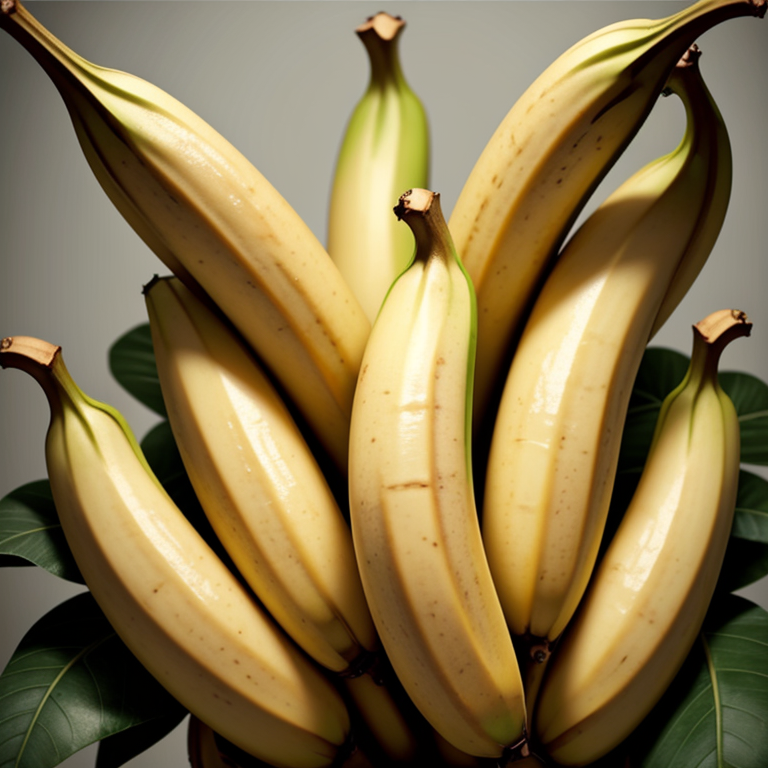
\includegraphics[width=0.6\textwidth]{files/ripe_bananas.png}
  \caption{\hebrewfont אשכול בננות בשלות המוכנות לקטיף, הממחיש את מראה הפרי.}
\end{figure}

תהליך הגידול והבשלת הבננות כולל מספר שלבים, מהפריחה ועד להתפתחות האשכולות והבשלתם.

\section{ערך תזונתי}
\addcontentsline{toc}{section}{ערך תזונתי} % Add the section to TOC

בננות נחשבות לפרי בריא ומזין במיוחד. הן מהוות מקור מצוין לפחמימות, אשלגן, ויטמין B6, ויטמין C וסיבים תזונתיים.

\begin{remarkBox}{הערה: בננות ואשלגן}
בננות מפורסמות במיוחד בזכות תכולת האשלגן הגבוהה שלהן. אשלגן הוא מינרל חשוב המסייע בוויסות לחץ הדם ובשמירה על תפקוד תקין של הלב והשרירים. בננה ממוצעת מכילה כ-\(400\) מ"ג אשלגן.
\end{remarkBox}

הערך הקלורי של בננה משתנה בהתאם לגודלה, אך בננה ממוצעת מכילה כ-\(105\) קלוריות. הן מספקות אנרגיה מהירה ולכן פופולריות בקרב ספורטאים.

\section{סוגים ושימושים}
\addcontentsline{toc}{section}{סוגים ושימושים} % Add the section to TOC

ישנם סוגים רבים של בננות, אך הסוג הנפוץ ביותר למאכל בעולם המערבי הוא בננת הקאבנדיש הצהובה. סוגים אחרים כוללים בננות אדומות, בננות תפוח ובננות פלנטיין, המשמשות לרוב לבישול או טיגון.

\begin{exampleBox}{דוגמה: שימושים נפוצים לבננות}
ניתן לצרוך בננות במגוון דרכים:
\begin{itemize}
    \item אכילה טרייה כחטיף.
    \item הוספה לשייקים ויוגורטים.
    \item שימוש במתכוני אפייה, כגון לחם בננות או עוגות.
    \item הכנת קינוחים קפואים.
\end{itemize}
\end{exampleBox}

\begin{figure}[H]
  \centering
  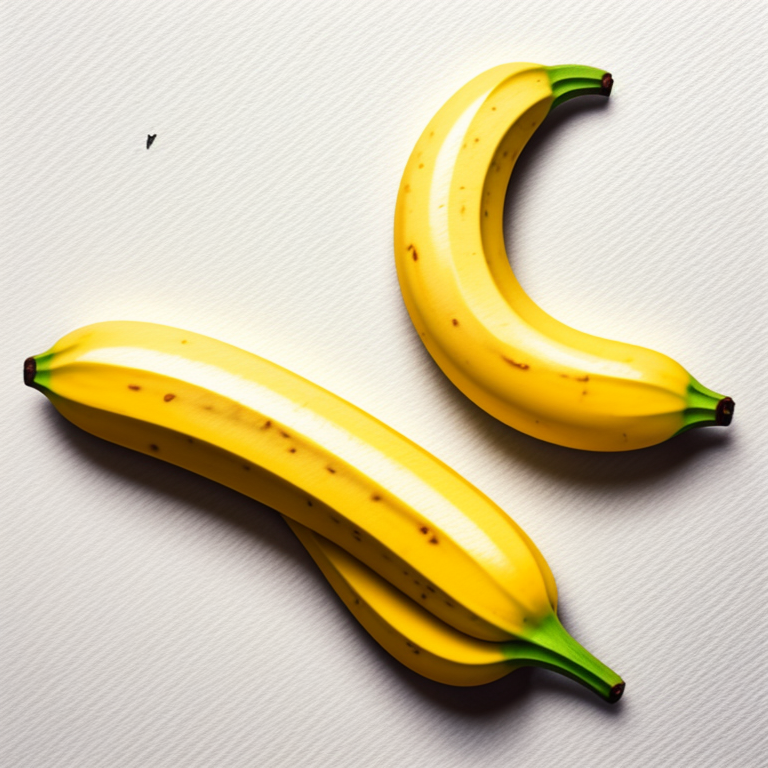
\includegraphics[width=0.4\textwidth]{files/peeling_banana.png}
  \caption{\hebrewfont המחשה ויזואלית לשימוש בבננה - קילוף קל ונוח לפני אכילה או שימוש.}
\end{figure}

\section*{סיכום}
\addcontentsline{toc}{section}{סיכום} % Add the unnumbered section to TOC

בננות הן פרי מזין, זמין ורבגוני, בעל היסטוריה ארוכה וחשיבות כלכלית ותזונתית ברחבי העולם. בין אם נאכלות טריות ובין אם משולבות במתכונים, הן מהוות תוספת מצוינת לתזונה בריאה.

\end{document}